%Elliptische Kurven


\chapter{Elliptische Kurven}
Als Basis für Asymentrische Kryptosysteme können elliptische Kurven dazu genutzt werden, die verschlüsselungstechnische Effektivität mathematischer Probleme, wie das des diskreten Logarithmus, zu erhöhen. Bei der Kryptographie unter Verwendung elliptsicher Kurven bei deutlich kürzerer Schlüssellänge ein gleichwertigers Ergebnis erzielt werden. Dieser Effekt wird durch die spezielle Arithmetik auf elliptischen Kurven erzielt, deren mathematische Grundlage, konkrete Eingenschaften und Funktionsweise im folgenden Kapitel erörtert werden soll.

Elliptische Kurven können über beliebigen Körpern definiert werden. Für die Kryptographie interessant sind elliptische Kurven über Primkörpern.

%\section{Definition: Elliptische Kurven}
% Sei \textit{p} eine \textit{Primzahl} $p>3$. Seien $a,b \in GF(p)$. Betrachte die Gleichung
%\begin{equation}
%    y^2 z = x^3 + axz^2 + bz^3.\label{eq:g1}
%\end{equation} Die \textit{Diskriminante}  dieser Gleichung ist
%\begin{equation}
%    \delta = -16(4a^3 + 27b^2).\label{eq:g2}
%\end{equation}
%Wir nehmen an, dass die Diskriminante $\delta$ nicht Null ist. Ist $(x,y,z) \in GF(p)^3$ eine Lösung dieser
%Gleichung, so ist für alle $c \in GF(p)$ auch $c(x,y,z)$ eine solche Lösung. Zwei Lösungen $(x,y,z)$ und $(x',y',z')$
%heißen \textit{äquivalent}, wenn es ein von Null verchiedenes $c \in GF(p)$ gibt mit $(x,y,z) = c(x',y',z')$. Dies
%definiert eine Äquivalenzrelation auf der Menge aller Lösungen der~\eqref{eq:g1}.




Um das weitere Verständnis zu verbessern, wollen wir uns erst eine uns schon bekannte Kurve ansehen. In Abbildung XY ist das Polynom $x^2 + y^2 = r^2$ über $\mathbb{R}$ dargestellt. Wie zu sehen ist, handelt es sich hierbei um die Kreisgleichung. Der zu sehende Kreis ist nichts anderes als die Menge aller Punkte, welche die Kreisgleichung erfüllen.
Ein Beispiel für eine solchen ist der Punkt $(r,0)$. Wenn $x$ den Wert $r$ hat, muss $y$ folglich den Wert $0$ haben. Ein Gegenbeispiel ist der Punkt $(r,r/2)$. Dieser erfüllt die Kreisgleichung nicht.
\begin{figure}[!h]
    \centering
    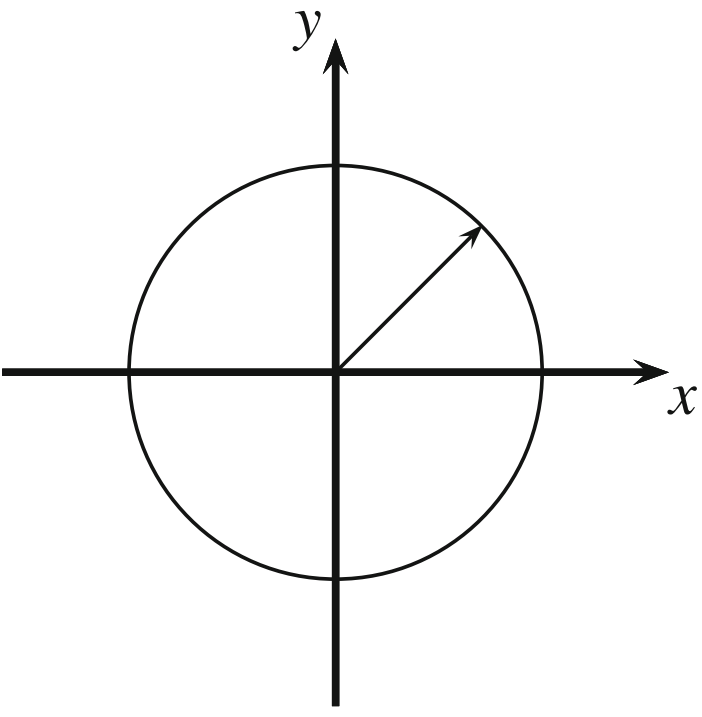
\includegraphics[width=0.3\textwidth]{grafiken/Kreis.PNG}
    \caption[r]{r}
    \label{fig:aufgaben_redesign}
\end{figure}
Die Kreisgleichung kann verallgemeinert werden, indem den Termen $x^2$ und $y^2$ Koeffizienten voran gesetzt werden. Eine solche Gleichung, $ax^2 + by^2 = c$ erzeugt über $\mathbb{R}$ eine Ellipse, wie in Abbildung XY zu sehen.
\begin{figure}[H]
    \centering
    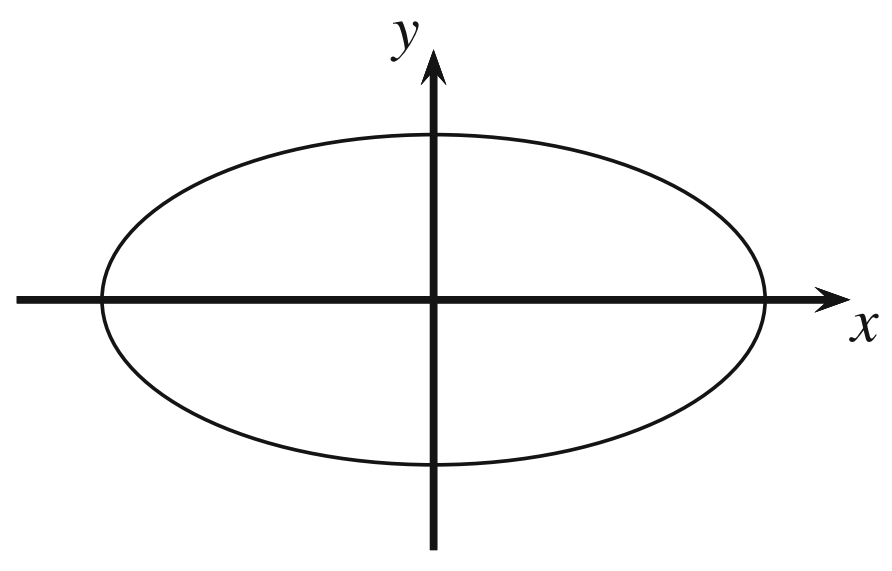
\includegraphics[width=0.3\textwidth]{grafiken/Ellipse.PNG}
    \caption[r]{r}
    \label{fig:aufgaben_redesign}
\end{figure}
Eine elliptische Kurve ist nun eine spezielle Polynomgleichung, der Form $y^2 = x^3 + ax + b$, unter der Bedingung $4a^3 + 27b^3 \neq 0$. Eine solche Gleichung über $\mathbb{R}$ ist in Abbildung XY dargestellt.
\begin{figure}[!h]
    \centering
    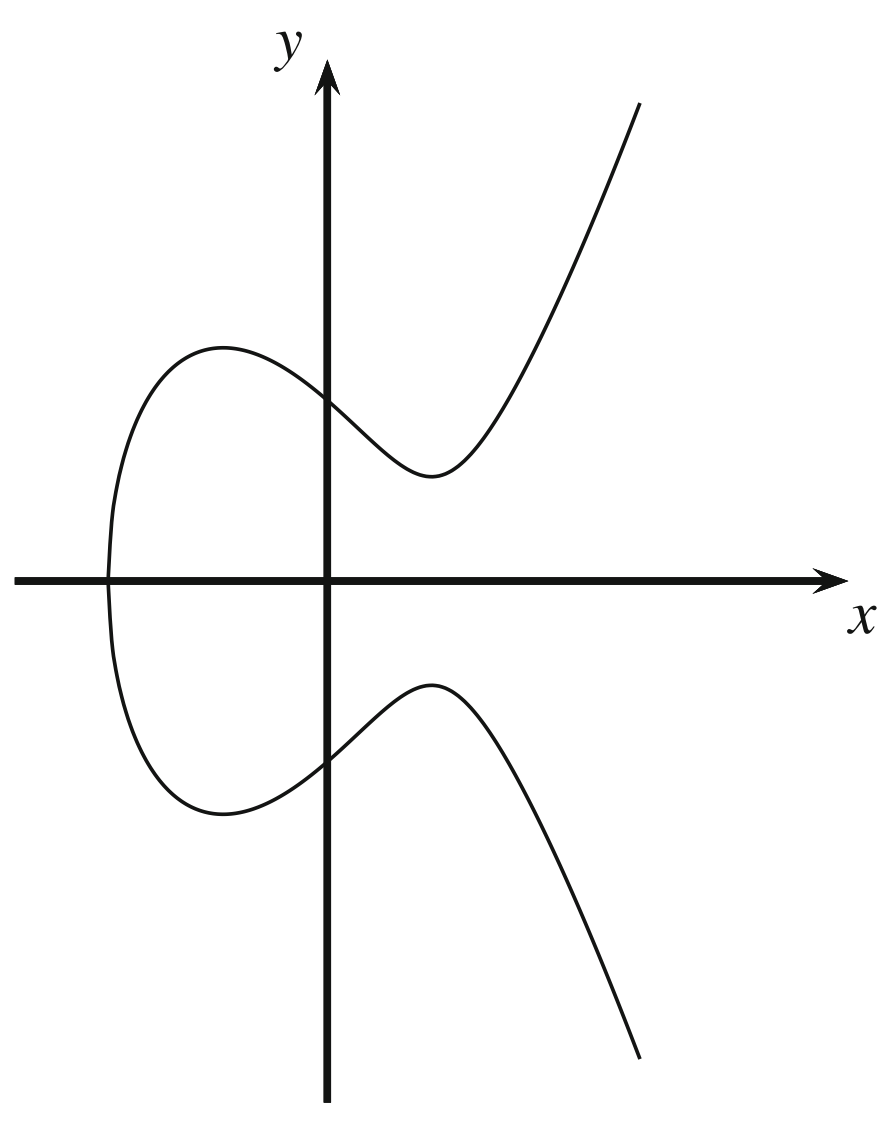
\includegraphics[width=0.3\textwidth]{grafiken/Elliptische_Kurve.PNG}
    \caption[r]{r}
    \label{fig:XXXX}
\end{figure}
Damit elliptische Kurven sinnvoll in der Kryptologie eingesetzt werden können, muss die Polynomgleichung über einem Primkörper betrachtet werden. Das heißt einfach gesprochen, alle Berechnungen werden modulo $p$ durchgeführt.
\paragraph{Definition: Elliptische Kurven über Primkörpern}
Die \textit{elliptische Kurve} über $mathbb{F_p}$, ist die Menge aller Punkte $(x,y)$ mit $x,y \in \mathbb{F_p}$, welche die folgende Gleichung erfüllen: 
\begin{center}
$y^2 \equiv x^3 + ax + b$ mod $p$, wobei $a,b \in \mathbb{F_p}$
\end{center} 
und die Bedingung  $$4a^3 + 27b^3 \neq 0$$ gelten müssen. Zu der elliptischen Kurve gehört des Weiteren auch der imaginäre \textit{Punkt im Unendlichen} $\mathcal{O}$.

Durch die Bedingung XY werden sog. Singularitäten ausgeschlossen. Andernfalls gäbe es Punkte, deren Tangente nicht wohldefiniert ist; letzteres ist aber für das Rechnen auf elliptischen Kurven erforderlich.

Elliptische Kurven über endlichen Körpern können grafisch nicht sinnvoll dargestellt werden. Ihre Form und Arithmetik lassen sich jedoch gut veranschaulichen wenn man sie auf $\mathbb{R}$ abbildet. Im Folgenden betrachten wir eine Elliptische Kurve, dargestellt in einem kartesischen Koordinatensystem, um die Gruppeneigenschaften bezüglich der Punktaddition zu zeigen.

Wie in Abbildung XY gezeigt, wird durch die zu addierenden Punkte $P$ und $Q$ eine Gerade gelegt, welche aufgrund der Kurveneigenschaften immer einen dritten Schnittpunkt mit der Kurve hat. Der $y$-Wert des Schnittpunktes wird im folgenden Schritt invertiert, wodurch der Punkt an der $x$-Achse gespieglt wird. Der aus diesen Schritten resultierende Punkt $R$ ist als Ergebnis der Addition auf der elliptischen Kurve definiert.

In dem grade betrachteten Fall ist $P \neq Q$, dieser wird Punktaddition genannt. Im Fall, dass $P = Q$ wird von der Punktverdopplung gesprochen.
























